%%%% Paramétrage du TD %%%%
\def\xxactivite{Activation\ifprof \\ \normalsize \vspace{-.4cm}Corrigé \else \fi}
\def\xxauteur{\textsl{Xavier Pessoles}}


%\def\xxnumchapitre{Chapitre 3 \vspace{.2cm}}
%\def\xxchapitre{\hspace{.12cm} Précision des systèmes}

\def\xxcompetences{%
\textsl{%
\textbf{Savoirs et compétences :}\\
\vspace{-.4cm}
%\begin{itemize}[label=\ding{112},font=\color{bleuxp}] 
%%\item \textit{Mod3.C2 : } pôles dominants et réduction de l’ordre du modèle : principe, justification
%%\item \textit{Res2.C4 : } stabilité des SLCI : définition entrée bornée -- sortie bornée (EB -- SB)	
%%\item \textit{Res2.C5 : } stabilité des SLCI : équation caractéristique	
%\item \textit{Res2.C6 : } stabilité des SLCI : position des pôles dans le plan complexe
%\item \textit{Res2.C7 : } stabilité des SLCI : marges de stabilité (de gain et de phase)
%\end{itemize}
}}


\def\xxfigures{
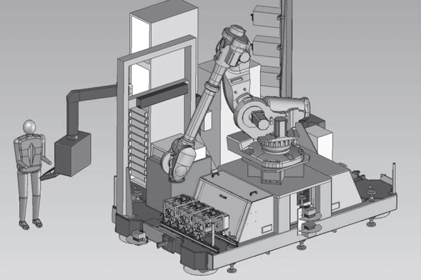
\includegraphics[width=.7\textwidth]{image1}
}%figues de la page de garde

\def\xxtitreexo{Cellule d'assemblage pour avion Falcon}
\def\xxsourceexo{D'après concours E3A -- PSI 2015.}

\input{\repRel/Style/pagegarde_TD}

\setlength{\columnseprule}{.1pt}

\pagestyle{fancy}
\thispagestyle{plain}


\vspace{4.5cm}

\def\columnseprulecolor{\color{bleuxp}}
\setlength{\columnseprule}{0.4pt} 

%%%%%%%%%%%%%%%%%%%%%%%


\begin{multicols}{2}
\setcounter{numques}{0}
\subsection*{Présentation}
Le tronçon central du fuselage du Falcon 7X est assemblé par rivetage grâce à un robot 6 axes. Les rivets sont stockés dans des cassettes rangées verticalement. Un chariot de sélection se déplace verticalement pour déplacer une buse d'aspiration qui permettra d'acheminer les rivets contenus dans la cassette vers l'effecteur (robot). Le chariot fait l'objet de cette étude.

\begin{center}
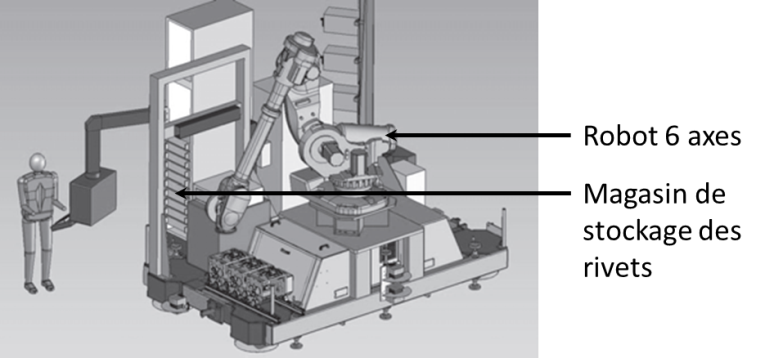
\includegraphics[width=7cm]{image5}
\end{center} 

\begin{obj}
Vérifier que les correcteurs proposés permettent ou non d'obtenir un écart statique nul et un écart en vitesse nul.
\end{obj}
% 
%L'objectif de cette partie est de valider les choix effectués par la société pour le sous ensemble de sélection des fixations de la cellule (exigence 1.1).

%\vfill
%
%\begin{center}
%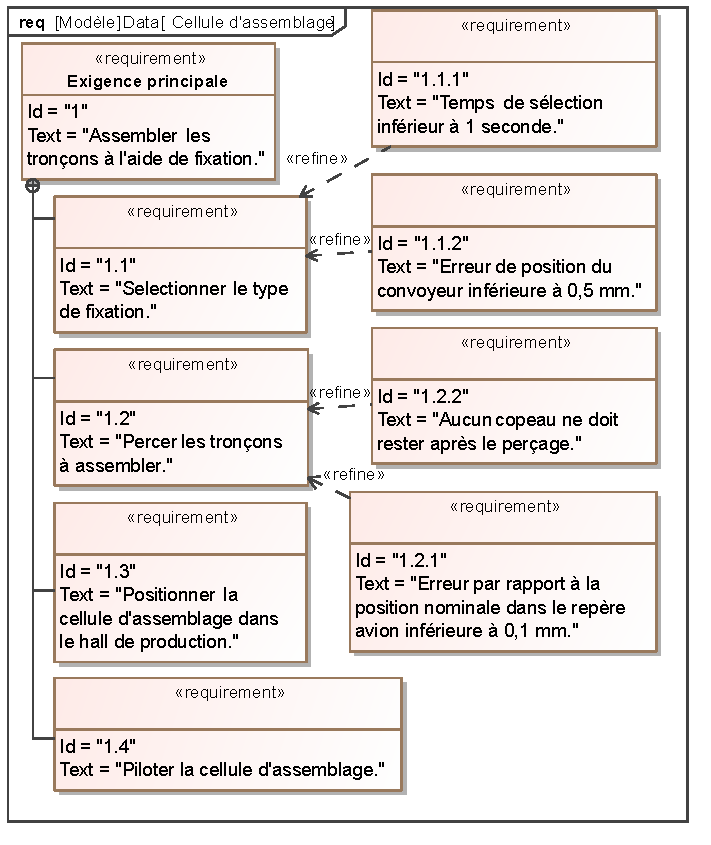
\includegraphics[width=7cm]{Exigences}
%\end{center} 




% 
%\subsection*{Axe chariot}
%Le déplacement du chariot est assuré par un axe numérique asservi en vitesse et en position. Cet axe est composé d'un moteur à courant continu, d'un système de transmission de puissance de type poulies / courroie et d'un rail.
% 
%\begin{center}
%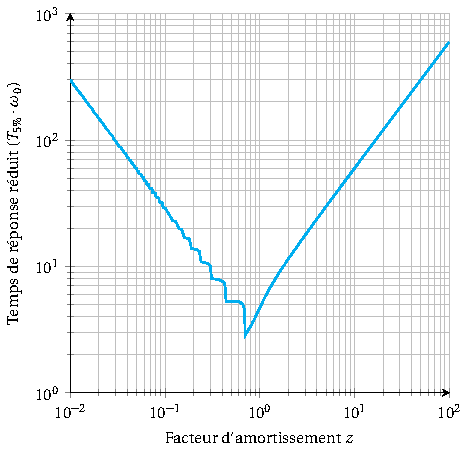
\includegraphics[width=4.5cm]{image7}
%\end{center} 
%
%
%\subsection*{Modélisation du système de déplacement du chariot}
%
%\begin{center}
%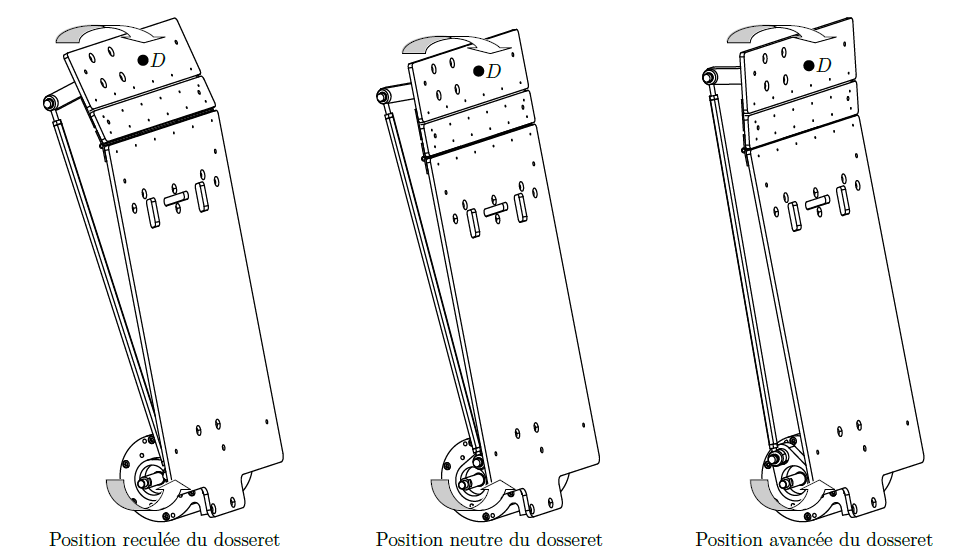
\includegraphics[width=5cm]{image8}
%\end{center} 
%
%
%\fi

%
%
%
%\section*{Sélectionner les fixations – Exigence 1.1}
%\ifprof
%\else 
%Afin de sélectionner le type de fixation, la buse d'aspiration doit être déplacée en face de la cassette avec une erreur inférieure à $\SI{0,5}{mm}$ (voir exigences fonctionnelles). Cependant le fabricant du système poulie-courroie du rail indique déjà une erreur de $\pm \SI{0,25}{mm}$ due notamment à l'élasticité de la courroie. Par conséquent, l'erreur en position de la commande doit être nulle. De plus, afin de ne pas perdre de temps lors de la production, le temps maximal de déplacement lors de la sélection est imposé à une seconde.
%
%L'étude se fera dans le cas le plus défavorable c'est-à-dire un déplacement du chariot vers le haut entre les deux cassettes de rivets les plus éloignées. L'axe de déplacement est appelé $\vect{y_c}$
%\subsection*{Notations domaine temporel – domaine de Laplace}
%
%Les notations entre le domaine temporel et celui de Laplace sont données dans la suite. Ainsi, si la fonction $f(t)$ possède une transformée de Laplace, elle sera notée : $F(p) = \mathcal{L}[f(t)]$.
%Les équations caractéristiques du moteur à courant continu sont rappelées ci-dessous (les conditions de Heaviside sont respectées) :
%\begin{itemize}[label=\ding{112},font=\color{ocre}] 
%\item $u(t)=e(t)+L \dfrac{di(t)}{\text{d} t}+Ri(t)$;
%\item $e(t)=K_E \omega_m (t)$ ;
%\item $C_M (t)=K_C i(t)$ ;
%\item $J_{eq}  \dfrac{d\omega_m)}{\text{d} t}+f\omega_m (t)=C_M (t)-C_R (t)$.
%\end{itemize}
%
%Avec : 
%\begin{itemize}[label=\ding{112},font=\color{ocre}] 
%\item $u(t)$ : tension moteur ;
%\item $i(t)$ : courant moteur ; 
%\item $e(t)$ : force contre-électromotrice ;
%\item $\omega_m(t)$ : vitesse de rotation moteur ;
%\item $C_M (t)$ : couple moteur ;
%\item $C_R (t)$: couple résistant modélisant l'action de pesanteur.
%\end{itemize}
%\fi
%
%\subsection*{Critères à respecter pour l'exigence 1.2}
%\ifprof
%\else
%\footnotesize{
%\begin{center}
%\begin{tabular}{|p{2cm}|p{2.5cm}|p{2cm}|}
%\hline
%Exigence	& Critères & Niveaux \\ \hline
%Déplacer le chariot	& Précision :
%erreur statique par rapport à une consigne de vitesse constante	
%& NULLE \\ \hline
%	& Rapidité : temps de réponse à 5\% en réponse à une consigne échelon 
%	& $Tr_{5\%} = \SI{0,1}{s}$  maxi \\ \hline
%	& Stabilité : & \\
%	& Marge de gain & \SI{6}{dB} mini \\
%	&Marge de gain & $\ang{45}$ mini \\
%\hline
%\end{tabular}
%\end{center}}

%\fi
%\subsection*{Choix d'une architecture de la chaine de transmission}
%\subparagraph{}
%\textit{Proposer sous la forme d'un schéma une autre solution permettant le déplacement du chariot. La conversion de l'énergie électrique en énergie mécanique par un moteur doit être conservée.}
%
%\ifprof
%\begin{corrige}
%Utilisation d’un système vis-écrou.
%\end{corrige}
%\else
%\fi
%
%\ifprof
%\else
%Compte tenu des vitesses de translation importantes, le système retenu est de type poulie-courroie.
%\fi
%
%\subsection*{Détermination de l'inertie équivalente} 
%\ifprof
%\else
%
%Les grandeurs caractéristiques (notations et valeurs) des éléments de l'axe du chariot sont données dans le tableau ci-dessous :
%\begin{center}
%\begin{tabular}{|p{3cm}|c|c|}
%\hline
%Moment d'inertie du rotor du moteur autour de son axe&	$J_m$ & $\num{140d-6}\si{kg.m^2}$ \\ \hline
%Moment d'inertie du réducteur ramené à l'arbre moteur&	$J_{réd}$ & $\num{60d-4}\si{kg.m^2}$ \\ \hline
%Moment d'inertie de la poulie motrice autour de son axe&	$J_{PM}$	&$ \num{38d-4}\si{kg.m^2}$ \\ \hline
%Moment d'inertie de la poulie réceptrice autour de son axe&	$J_{PR}$ & $\num{38d-4}\si{kg.m^2}$ \\ \hline
%Masse totale du chariot	&$M$ &$\SI{5}{kg}$ \\ \hline
%Vitesse de rotation de l'arbre moteur &$\omega_m$ &  \\ \hline
%Vitesse de rotation de l'arbre de sortie du réducteur	&$\omega_r$&  \\ \hline
%Rayon d'une poulie motrice ou réceptrice	& $R_P$ &$\SI{45}{mm}$ \\ \hline
%Rapport de réduction réducteur ($\omega_r/\omega_m$)	& $\lambda$	&$1/5$ \\ \hline
%\end{tabular}
%\end{center}
%\fi
%
%\subparagraph{}
%\textit{À partir des grandeurs définies déterminer l'expression littérale de l'inertie équivalente $J_{eq}$ de l'ensemble $\Sigma=$\{moteur+réducteur+poulies+chariot\} ramenée sur l'arbre moteur. Cette inertie équivalente est définie par $E_c (\Sigma)=1/2 J_{eq} \omega_m^2$.}
%\ifprof
%\begin{corrige}
%$\mathcal{E}_c(\Sigma)=\mathcal{E}_c (\text{moteur})+\mathcal{E}_c (\text{réducteur})+\mathcal{E}_c (\text{poulies})+\mathcal{E}_c (\text{chariot})$.
%\begin{itemize}
%	\item $\mathcal{E}_c (\text{moteur})=1/2 J_m \omega_m^2$;
%	\item $\mathcal{E}_c (\text{réducteur})=1/2 J_{\text{red}} \omega_m^2$;
%	\item $\mathcal{E}_c (\text{poulies})=1/2 (J_{\text{Pm}}+J_{\text{PR}}  ) \omega_{\text{red}}^2=1/2 (J_{\text{Pm}}+J_{\text{PR}}  ) \lambda^2 \omega_m^2$;
%	\item $\mathcal{E}_c (\text{chariot})=1/2 MV^2=1/2 MR_p^2 \lambda^2 \omega_m^2$.
%\end{itemize}
%On a donc $J_{\text{eq}}=MR_p^2 \lambda^2+(J_{\text{Pm}}+J_{\text{PR}}  ) \lambda^2+J_{\text{red}}+J_m$.
%
%\end{corrige}
%\else
%\fi
%
%\subparagraph{}
%\textit{Déterminer la valeur numérique de l'expression précédente.}
%\ifprof
%\begin{corrige}
%$J_{eq}=\SI{0,0068}{kg.m^2}$
%\end{corrige}
%\else
%\fi
%
%\subsection*{Modèle de connaissance du moteur à courant continu}
%
%\begin{obj}
%L'objectif de cette partie est d'établir un modèle de la motorisation de l'axe afin de simuler un déplacement.
%\end{obj}
%
%\subparagraph{}
%\textit{À partir des équations du moteur à courant continu, réaliser le schéma bloc du moteur à courant continu.}
%\ifprof
%\begin{corrige} ~\\
%
%\begin{center}
%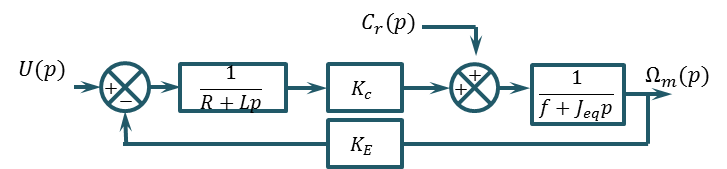
\includegraphics[width=7cm]{corr_01}
%\end{center} 
%\end{corrige}
%\else
%\fi
%
%\subparagraph{}
%\textit{En considérant que $C_R (p)=0$, déterminer la fonction de transfert $H_M (p)=\dfrac{\Omega_m (p)}{U(p)}$ sous sa forme canonique.}
%\ifprof
%\begin{corrige}
%$H_m (p)=\dfrac{\dfrac{K_C}{K_c K_E+Rf}}{1+\dfrac{RJ_eq+Lf}{K_c K_E+Rf}p+\dfrac{LJ_eq}{K_c K_E+Rf} p^2}$
%\end{corrige}
%\else
%\fi
%
%\subparagraph{}
%\textit{Montrer que la fonction de transfert $H_M (p)$ peut se mettre sous la forme $H_M (p)=\dfrac{K_C}{K_C K_e+RJ_{eq} p+LJ_{eq} p^2 }$. Justifier la réponse. Pour cette question, la valeur numérique de $J_{eq}$ considérée sera $J_{eq}=\num{7d-3}\si{kg.m^2}$ indépendamment du résultat numérique calculé précédemment.}
%\ifprof
%\begin{corrige}
%En faisant les applications numériques on montre que $Rf$ est négligeable devant $K_c K_E$ et que $Lf$ et négligeable devant $RJ_{eq}$. On a donc : 
%$H_m (p)=\dfrac{\dfrac{K_C}{K_c K_E}}{1+\dfrac{RJ_{eq}}{K_c K_E }p+\dfrac{LJ_{eq}}{K_c K_E }p^2 }=\dfrac{K_C}{K_c K_E+RJ_{eq} p+LJ_{eq} p^2 }$.
%
%\end{corrige}
%\else
%\fi
%
%\subparagraph{}
%\textit{Montrer qu'avec l'expression, $H_M (p)$ peut s'écrire sous la forme $H_M (p)=\dfrac{K_M}{(1+T_E p)(1+T_M p)}$  avec $T_E<T_M$.}
%\ifprof
%\begin{corrige}
%$
%\left\{
%\begin{array}{l}
%T_e+T_m= \dfrac{RJ_{eq}}{K_c K_e}\\
%T_e T_m=\dfrac{LJ_{eq}}{K_C K_e}
%\end{array}
%\right.
%$
%On a (résolution d’une équation du second degré):
%
%$Te=\dfrac{\dfrac{RJ_{eq}}{K_c K_e}-\sqrt{\left(\dfrac{RJ_{eq}}{K_c K_e}\right)^2 - 4\dfrac{LJ_{eq}}{K_c K_e}}}{2}$. $T_e=\SI{0,0051}{s}$ et $T_m=\SI{0,0074}{s}$.
%
%
%\end{corrige}
%\else
%\fi
%\section*{Étude de l'asservissement en position de l'axe}
%\subsection*{Modélisation de l'asservissement en position}
%\ifprof
%\else
%
%
%La partie précédente a permis de déterminer un modèle du moteur. La suite de l'étude va permettre, par simulation, de déterminer les réglages nécessaires de l'axe vis-à-vis du cahier des charges. La figure suivante présente le principe de l'asservissement de l'axe du chariot.
% 
%\begin{center}
%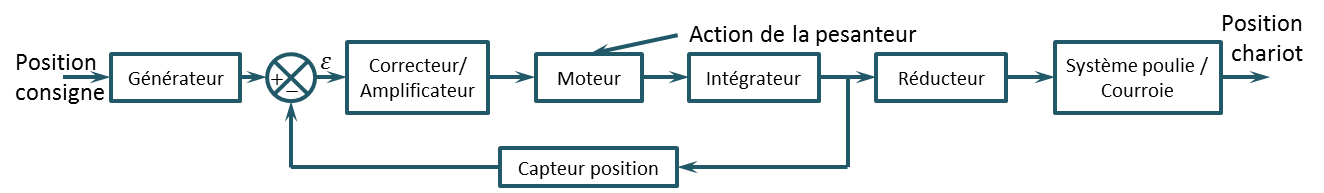
\includegraphics[width=7cm]{image9}
%\end{center} 
%
%Les grandeurs caractéristiques des blocs de l'asservissement de l'axe chariot sont données dans le tableau ci-dessous :
%\begin{center}
%\begin{tabular}{|c|c|c|}
%\hline
%Générateur & $K_G$ & À déterminer \\
%\hline
%Capteur de position	& $K_\text{capt}$ & $\num{5d-3}\si{V.rad^(-1)}$ \\
%\hline
%Correcteur amplificateur	 & $C(p)$ & Variable \\
%\hline
%\end{tabular}
%\end{center}
%\fi
%
%\subparagraph{}
%\textit{Quelle doit être la valeur de $K_G$ pour assurer un asservissement correct (c'est-à-dire l'écart $\varepsilon$ doit être nul si la position de l'axe est identique à la consigne) ?}
%\ifprof
%\begin{corrige} ~\\
%
%On doit avoir $K_G=K_{\text{capt}} \dfrac{1}{\lambda} \dfrac{1}{R_p}=\SI{0,556}{V.rad^{-1}.m^{-1}}$.
%\end{corrige}
%\else
%\fi
%
%\subparagraph{}
%\textit{Donner le schéma-blocs de l'asservissement.}
%\ifprof
%\begin{corrige} ~\\
%
%\begin{center}
%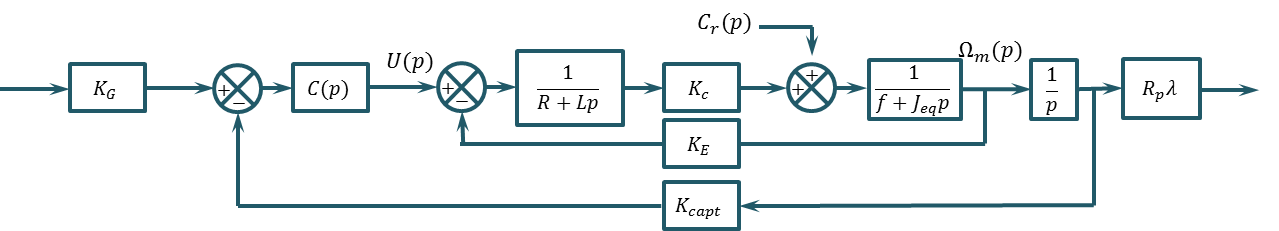
\includegraphics[width=7cm]{corr_02}
%\end{center} 
%
%\end{corrige}
%\else
%\fi

\subsection*{Étude du modèle simplifié}
\ifprof
\else
Afin de faciliter les calculs, le schéma bloc à retour unitaire est donné figure suivante. Le couple résistant $C_r$ dû à l'action de pesanteur est supposé constant.
 
 \begin{center}
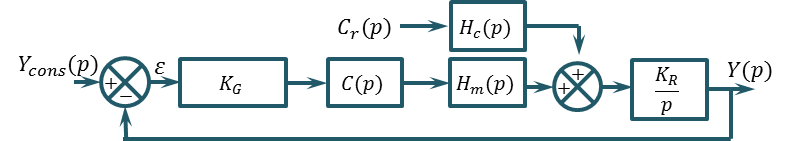
\includegraphics[width=\linewidth]{image10}
\end{center} 


Avec : 

\noindent $H_M (p)=\dfrac{K_M}{(1+T_E p)(1+T_M p)} \text{ et }
H_C (p)=\dfrac{\dfrac{\left(R+Lp\right)K_M}{K_C}}{(1+T_E p)(1+T_M p)}$.
%\item $C_R (p)=C_r/p$;
%\item $K_R=R_p \lambda$.
%\end{itemize}
\fi

\subsection*{Etude du modèle sans perturbation}

\question{On souhaite déterminer l'erreur en position du système. Calculer l'écart statique pour $C(p)=K_p$. Pouvait-on prévoir le résultat ?}
\ifprof
\begin{corrige}
\end{corrige}
\else
\fi

\question{On souhaite déterminer l'erreur en vitesse du système. Calculer l'écart statique pour $C(p)=\dfrac{K_i}{p}$. Pouvait-on prévoir le résultat ?}
\ifprof
\begin{corrige}
\end{corrige}
\else
\fi



\subsection*{Etude du modèle avec perturbation}

\question{Donner l'expression de $\varepsilon(p)$.}
\ifprof
\begin{corrige}~\\
On raisonne par superposition :

Si $C_r (p)=0$: 

$$Y_1 (p)
=Y_{\text{cons}}(p) \dfrac{\dfrac{K_G K_{\text{Capt}} C(p) H_m (p) K_r}{p}}{1+\dfrac{K_G K_{\text{Capt}} C(p) H_m (p) K_r}{p}}$$

$$
=Y_{\text{cons}} (p) \dfrac{K_G K_{\text{Capt}} C(p) H_m (p) K_r}{p+K_G K_{\text{Capt}} C(p) H_m (p) K_r } 
$$

$$
=Y_{\text{cons}} (p) \dfrac{K_G K_{\text{Capt}} C(p) K_M  K_r}{(1+T_E p)(1+T_M p)p+K_G K_{\text{Capt}} C(p) K_M K_r )}$$.

\end{corrige}

\begin{corrige}
Si $Y_{\text{Cons}} (p)=0$ :

$$Y_2 (p)
=C_r (p) \dfrac{\dfrac{H_c (p) K_r}{p}}{1+\dfrac{K_r K_G K_{\text{Capt}} C(p) H_m (p)}{p} }$$

$$
=C_r (p) \dfrac{H_c (p) K_r}{p+K_r K_G K_{\text{Capt}} C(p) H_m (p) }$$
$$
=C_r (p) \dfrac{\dfrac{(R+Lp) K_M  K_r}{K_C }}{(1+T_E p)(1+T_M p)p+K_r K_G K_{\text{Capt}} C(p) K_M }$$

On a donc :
$Y(p)=Y_1 (p)+Y_2 (p)$.

\end{corrige}
\else
\fi

\question{On souhaite déterminer l'erreur en position du système. Calculer l'écart statique pour $C(p)=K_p$. Pouvait-on prévoir le résultat ?}
\ifprof
\begin{corrige}
\end{corrige}
\else
\fi


\question{On souhaite déterminer l'erreur en position du système. Calculer l'écart statique pour $C(p)=\dfrac{K_i}{p}$. Pouvait-on prévoir le résultat ?}
\ifprof
\begin{corrige}
\end{corrige}
\else
\fi


\question{On souhaite déterminer l'erreur en vitesse du système. Calculer l'erreur pour $C(p)=\dfrac{K_i}{p}$. Pouvait-on prévoir le résultat ?}
\ifprof
\begin{corrige}
\end{corrige}
\else
\fi


\question{On souhaite déterminer l'erreur pour un entrée en position du système avec une perturbation de type rampe. Calculer l'erreur pour $C(p)=\dfrac{K_i}{p}$. Pouvait-on prévoir le résultat ?}
\ifprof
\begin{corrige}
\end{corrige}
\else
\fi

%
%\subparagraph{}
%\textit{On souhaite que lorsque le système se déplace à vitesse constante, l'erreur sur la vitesse atteinte par le système soit nulle. Quelle sollicitation doit-on utiliser. Calculer l'écart statique pour $C(p)=K_p$ puis $C(p)=\dfrac{K_i}{p}$.}
%\ifprof
%\begin{corrige}
%\end{corrige}
%\else
%\fi
%
%\subparagraph{}
%\textit{Conclure.}
%\ifprof
%\begin{corrige}
%\end{corrige}
%\else
%\fi

%\ifprof
%\else
%
%Afin de répondre totalement au cahier des charges, l'utilisation d'un correcteur proportionnel intégral dérivé est retenue. En effet, la commande de l'axe intègre directement ce type de correcteur. Dans la suite du problème, le correcteur $C(p)$ sera de la forme : $C(p)=K_I \left(1+\dfrac{1}{(T_I p}\right)\left(1+T_D p\right)$. Le réglage des coefficients a été fait par simulation numérique.
%Afin de vérifier maintenant le critère de rapidité, on donne la réponse temporelle (figure page suivante) de l'axe à un échelon de position de $\SI{1}{m}$.
%
%\fi
%
%\subparagraph{}
%\textit{Conclure sur la conformité au cahier des charges du système ainsi réglé.}
%\ifprof
%\begin{corrige}
%\end{corrige}
%\else
%\fi
%
%\ifprof
%\else
% 
% \begin{center}
%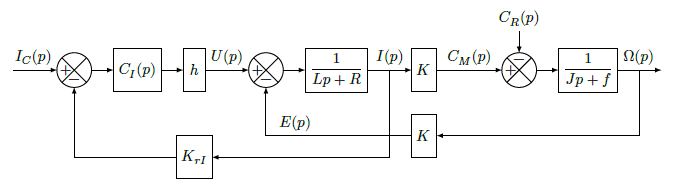
\includegraphics[width=7cm]{image11}
%\end{center} 
%
%\fi
% 
%
%\subparagraph{}
%\textit{Tracer de diagramme de Bode.}
%\ifprof
%\begin{corrige}
%\end{corrige}
%\else
%\fi
%
%\ifprof
%\else
%
%On considère $C_R (p)=0$. On prendra $K_M=\SI{0,8}{rad.s^{-1}.V^{-1}}$, $T_e=\SI{0,0051}{s}$,$T_m=\SI{0,0074}{s}$.
%\fi
%
%\subparagraph{}
%\textit{Tracer le diagramme de Bode de la fonction de transfert en boucle ouverte pour $C(p)=1$. Déterminer les marges de phase et les marges de gain.}
%\ifprof
%\begin{corrige}
%\end{corrige}
%\else
%\fi
% 
%\subparagraph{}
%\textit{Tracer le diagramme de Bode de la fonction de transfert en boucle ouverte pour $C(p)=\dfrac{1}{p}$. Déterminer les marges de phase et les marges de gain.}
%\ifprof
%\begin{corrige}
%\end{corrige}
%\else
%\fi
%
%\ifprof
%\else
%
%On donne ci-dessous les diagrammes de Bode avec les correcteurs optimisés. Déterminer les marges de gain et marges de phase. 
%\fi
%
%\section*{Vérification des performances de l'axe du magasin de rivets}
%\ifprof
%\else
%
%Afin de vérifier les réglages précédents, un essai sur le système réel est réalisé. Une consigne de \SI{2}{m} est donnée. L'absence de système d'acquisition dédié impose un système de mesure extérieur au système réel. C'est un dispositif d'analyse d'image qui est retenu pour ces mesures.
%\fi
%
%\subparagraph{}
%\textit{À partir des relevés ci-dessous, conclure sur le respect des exigences fonctionnelles de l'axe du magasin de stockage des rivets (Exigence 1.1).}
%\ifprof
%\begin{corrige}
%\end{corrige}
%\else
%\fi
 
\end{multicols}
%
%\ifprof
%\else
%
%\begin{center}
%\begin{tabular}{cc}
%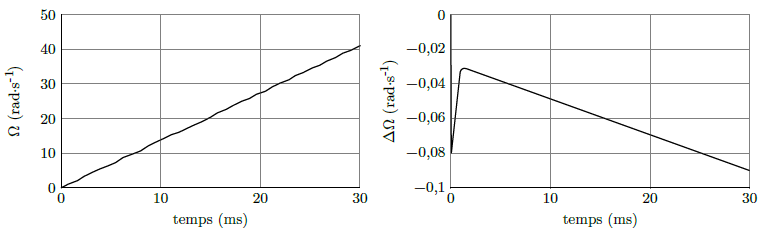
\includegraphics[width=7cm]{image13} &
%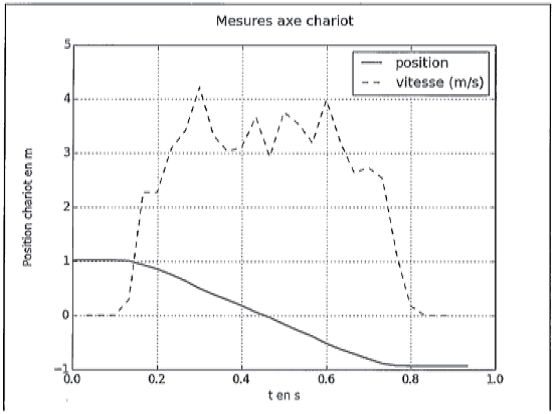
\includegraphics[width=7cm]{image14}
%
%\end{tabular}
%\end{center}
%
% \begin{center}
%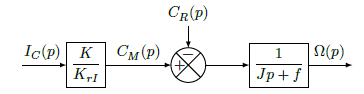
\includegraphics[width=\textwidth]{image12}
%\end{center} 
%\fi

%\end{document}
